

%%
%% The "title" command has an optional parameter,
%% allowing the author to define a "short title" to be used in page headers.
\title{Neural Machine Translation With Imbalanced Classes}
\titlenote{This work has been published at \textit{Findings of the Association for Computational Linguistics: EMNLP 2020} with title ``Finding the optimal vocabulary size for neural machine translation." }

%%
%% The "author" command and its associated commands are used to define
%% the authors and their affiliations.
%% Of note is the shared affiliation of the first two authors, and the
%% "authornote" and "authornotemark" commands
%% used to denote shared contribution to the research.
\author{Thamme Gowda}
%\authornote{}
\email{tg@isi.edu}
\email{tnarayan@usc.edu}
%\orcid{1234-5678-9012}

\affiliation{%
  \institution{Dept. of Computer Science,
   University of Southern California, Los Angeles, CA, USA}
  %\streetaddress{P.O. Box 1212}
  \city{Los Angeles}
  \state{CA}
  \postcode{90089}
}


%%
%% By default, the full list of authors will be used in the page
%% headers. Often, this list is too long, and will overlap
%% other information printed in the page headers. This command allows
%% the author to define a more concise list
%% of authors' names for this purpose.
\renewcommand{\shortauthors}{Gowda}


%%
%% The code below is generated by the tool at http://dl.acm.org/ccs.cfm.
%% Please copy and paste the code instead of the example below.
%%
\begin{CCSXML}
<ccs2012>
    <concept>
       <concept_id>10010147.10010257</concept_id>
       <concept_desc>Computing methodologies~Machine learning</concept_desc>
       <concept_significance>500</concept_significance>
       </concept>
   <concept>
       <concept_id>10010147.10010178.10010179</concept_id>
       <concept_desc>Computing methodologies~Natural language processing</concept_desc>
       <concept_significance>500</concept_significance>
       </concept>
   <concept>
       <concept_id>10010147.10010178.10010179.10010180</concept_id>
       <concept_desc>Computing methodologies~Machine translation</concept_desc>
       <concept_significance>500</concept_significance>
       </concept>
   <concept>
       <concept_id>10010147.10010178.10010179.10010182</concept_id>
       <concept_desc>Computing methodologies~Natural language generation</concept_desc>
       <concept_significance>500</concept_significance>
       </concept>
 </ccs2012>
\end{CCSXML}

\ccsdesc[500]{Computing methodologies~Natural language processing}
\ccsdesc[500]{Computing methodologies~Natural language generation}
\ccsdesc[500]{Computing methodologies~Machine translation}
\ccsdesc[500]{Computing methodologies~Machine learning}

%%
%% Keywords. The author(s) should pick words that accurately describe
%% the work being presented. Separate the keywords with commas.
\keywords{Zipfian long tail, Rare phenomenon learning, Imbalanced learning}



%% A "teaser" image appears between the author and affiliation
%% information and the body of the document, and typically spans the
%% page.

%\begin{teaserfigure}
%  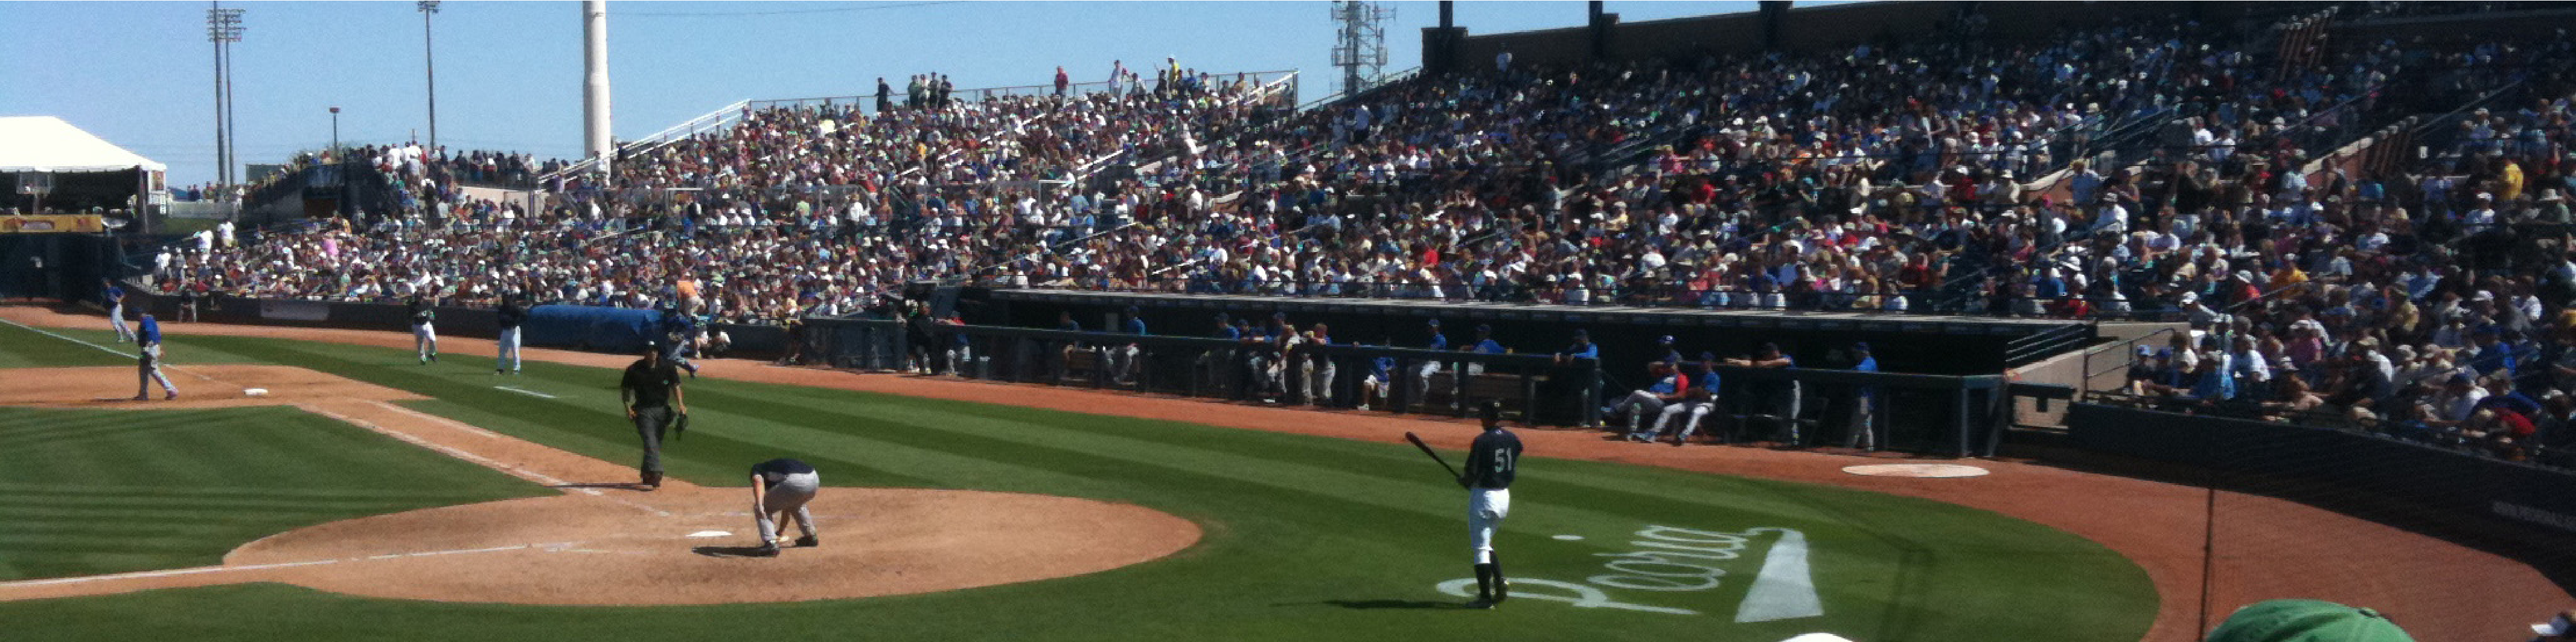
\includegraphics[width=\textwidth]{sampleteaser}
%  \caption{Seattle Mariners at Spring Training, 2010.}
%  \Description{Enjoying the baseball game from the third-base
%  seats. Ichiro Suzuki preparing to bat.}
%  \label{fig:teaser}
%\end{teaserfigure}



%%%%%% these are alias to ACL commands

\newcommand{\newcite}{\citet}
%% \newcommand{\citet}{\cite}
%% \newcommand{\citep}{\cite}


\newcommand{\bleu}{{\textsc{Bleu}}}
\newcommand{\chrf}[1]{\textsc{ChrF}{$_{#1}$}}

\newcommand{\maf}[1]{\textsc{MacroF}{\text{$_{{#1}}$}}}
\newcommand{\mif}[1]{\textsc{MicroF}{\text{$_{{#1}}$}}}

\newcommand{\blrtmn}{\textsc{BLEURT}\text{\footnotesize{}mean}}
\newcommand{\blrtmd}{\textsc{BLEURT}\text{\footnotesize{}median}}

\newcommand{\insig}{$^{\times}$}
\newcommand{\myurl}[1]{\href{#1}{#1}}

